%%% Template originaly created by Karol Kozioł (mail@karol-koziol.net) and modified for ShareLaTeX use

\documentclass[a4paper,fleqn,11pt]{article}

\usepackage[T1]{fontenc}
\usepackage[utf8]{inputenc}
\usepackage{graphicx}
\usepackage{xcolor}

\usepackage{tgtermes}

\usepackage[
pdftitle={EE698G - Probabilistic Mobile Robotics Assignment}, 
pdfauthor={Satya Prakash Panuganti, 14610},
colorlinks=true,linkcolor=blue,urlcolor=blue,citecolor=blue,bookmarks=true,
bookmarksopenlevel=2]{hyperref}
\usepackage{amsmath,amssymb,amsthm,textcomp}
\usepackage{enumerate}
\usepackage{multicol}
\usepackage{tikz}

\usepackage{geometry}
\geometry{total={210mm,297mm},
left=25mm,right=25mm,%
bindingoffset=0mm, top=20mm,bottom=20mm}

\usepackage{ mathrsfs }
\usepackage{ upgreek }
\linespread{1.3}

\newcommand{\linia}{\rule{\linewidth}{0.5pt}}

% custom theorems if needed
\newtheoremstyle{mytheor}
    {1ex}{1ex}{\normalfont}{0pt}{\scshape}{.}{1ex}
    {{\thmname{#1 }}{\thmnumber{#2}}{\thmnote{ (#3)}}}

\theoremstyle{mytheor}
\newtheorem{defi}{Definition}

% my own titles
\makeatletter
\renewcommand{\maketitle}{
\begin{center}
\vspace{2ex}
{\huge \textsc{\@title}}
\vspace{1ex}
\\
\linia\\
\@author \hfill \@date
\vspace{4ex}
\end{center}
}
\makeatother
%%%

% custom footers and headers
\usepackage{fancyhdr,lastpage}
\pagestyle{fancy}
\lhead{}
\chead{}
\rhead{}
\lfoot{Assignment 3}
\cfoot{}
\rfoot{Page \thepage\ /\ \pageref*{LastPage}}
\renewcommand{\headrulewidth}{0pt}
\renewcommand{\footrulewidth}{0pt}
%

%%%----------%%%----------%%%----------%%%----------%%%

\begin{document}

\title{EE698G - Probabilistic Mobile Robotics Assignment}

\author{Satya Prakash Panuganti, 14610}

\date{19 February, 2017}

\maketitle

\section{}

Let `E' be the event that the first coin (biased one), on flipping it twice, shows heads both times. \\
Let `F' be the event theat the second coin (unbiased one), on flipping it twice, shows heads both times. \\
Let `B' be the event that the biased coin is chosen and `C' be the event that the unbiased coin is chosen. \\
Let 'H' be the event that on selecting a coin at random and flipping it, heads are observed in both tosses.
\begin{align*}
\ We\ have,\ P(B) = P (C) & = 0.5 \\
\because\ P(Heads) & = 0.6\ for\ the\ biased\ coin\ :\\
P (E) & = 0.6 \times 0.6 \\
& = 0.36 \\
Similarily,\ for\ the\ unbiased\ coin\ : \\
P (F) & = 0.5 \times 0.5 \\
& = 0.25 \\
Now,\ P (B | H) & = \frac{P (B \cap H)}{P (H)} \\
P (B \cap H) & = P (B \cap E) & \because\ B \cap H = B \cap E \\
& = P (B) \times P (E) & \because\ events\ B\ and\ E\ are\ independent \\
& = 0.5 \times 0.36 \\
& = 0.18 \\
Now,\ P (H) & = P (H \cap B) + P (H \cap C)\ & Using\ Total\ Probability\ Theorem\ \\
 & & \because\ B\ \&\ C\ are\ mutually \\
 & &  exclusive\ and\ exhaustive. \\
 & = P (B \cap E) + P (C \cap F) & \because\ B \cap H = B \cap E\ \&\ C \cap H = C \cap F\ \\
 & = 0.18 + P (C) \times p (F) & \because\ events\ C\ and\ F\ are\ independent \\
 & = 0.18 + 0.5 \times 0.25 \\\
 & = 0.18 + 0.125 \\
 & = 0.305 \\
 \therefore\ P (B | H) & = \frac{P (B \cap H)}{P (H)} \\
 & = \frac{0.18}{0.305} \\
 & = 0.59
\end{align*}

\section{}

Let $S_B$ be the event that the car appears blue and $S_G$ be the event that the car apprears to be green. \\
Let $G$ be the event that the car is green and $B$ be the event that the car is blue.
\begin{align*}
Now,\ P (B | S_B) & = \frac{P (S_B | B) P (B)}{P (S_B)} \\
\&\ P (G | S_G) & = \frac{P (S_G | G) P (G)}{P (S_B)}
\end{align*}
If we do not know the value of P (B) and P (G), it is not possible to calculate the most likely color of the taxi. \\

With the information, \textbf{`9 out of 10 Athenian taxi are green'}, we have, \\
$P (B) = 0.1\ \&\ P (G) = 0.9$ \\

It is clear to me that the statement \textbf{`discrimination between blue and green is 75\% reliable'} implies that $P (B \cap S_B) + P (G \cap S_G) = 0.75$.

\subsection*{Case 1}
If the statement, \textbf{`discrimination between blue and green is 75\% reliable'} \textbf{does not mean} that $P(S_B | B) = P (S_G | G)$, then it is not possible to calculate the most likely color of the taxi.

\subsection*{Case 2}
However, if the statment, \textbf{`discrimination between blue and green is 75\% reliable', does imply} that $P(S_B | B) = P (S_G | G)$, then it becomes possible to calculate the most likely color of the taxi.

\begin{align*}
Now,\ P (B \cap S_B) + P (G \cap S_G) = 0.75. \\
\implies\ P (S_B | B) P (B) + P (S_G | G) P (G) = 0.75 \\
\implies\ P (S_B | B) (P (B) + P (G)) = 0.75 \\
\implies\ P (S_B | B) \times 1 = 0.75 \\
\implies\ P (S_B | B)  = 0.75\ \&\ P (S_G | G) = 0.75
\end{align*}

\begin{align*}
Also,\ P (S_B | G) & = \frac{P (S_B \cap G)}{P (G)} \\
& = \frac{P (G) - P (S_G \cap G)}{P (G)}\ &\
\because [G = (S_G \cap G) \cup (S_B \cap G)\ \&\ 
\phi = (S_G \cap G) \cap (S_B \cap G)] \\
& = 1 - \frac{P (S_G \cap G)}{P (G)} \\
& = 1 - P (S_G | G) \\
& = 0.25
\end{align*}

\begin{align*}
Now,\ P (B | S_B) & = \frac{P (S_B | B) P (B)}{P (S_B)} \\
& = \frac{0.75 \times 0.1}{P (S_B)} \\
& = 0.075\eta,\ where\ \eta = \frac{1}{P (S_B)} \\
Also,\ P (G | S_B) & = \frac{P (S_B | G) P (G)}{P (S_B)} \\
& = \frac{0.25 * 0.9}{P (S_B)} \\
& = 0.225\eta \\
We\ have, P (B|S_B) + P (G|S_B) & = \frac{P (B \cap S_B) + P (G \cap S_B}
										  {P (S_B)} \\
& = \frac{P (S_B)}{P (S_B)} \\
& = 1. \\
\therefore\ 0.225\eta + 0.075\eta & = 1 \\
\implies\ 0.3\eta & = 1 \\
\eta & = 3.33 \\
\therefore\ P (B|S_B) & = 3.33 \times 0.075 \\
& = 0.25 \\
\&\ P (G|S_B) & = 3.33 \time 0.225 \\
& = 0.75 \\
Hence,\ P (G|S_B) > P (B|S_B)
\end{align*}
$\therefore$ The most likely color of the taxi is green.
\section{}

\begin{align*}
P (X, Y) &  = \frac{1}{2\pi \sqrt{|\Sigma|}}exp \begin{Bmatrix}
		      -\frac{1}{2}
  		   	  \begin{bmatrix}
				X - \mu_X \\
				Y - \mu_y
			  \end{bmatrix}^T
		   	  \Sigma^{-1}
		      \begin{bmatrix}
		   		X - \mu_X \\
				Y - \mu_y
			  \end{bmatrix} \end{Bmatrix} \\
Now,\ P (Y = y) & = \int_{-\infty}^{\infty} P (X = x, Y = y) dx \\
& = \int_{-\infty}^{\infty}
			  \frac{1}{2\pi \sqrt{|\Sigma|}}exp \begin{Bmatrix}
		      -\frac{1}{2}
  		   	  \begin{bmatrix}
				x - \mu_X \\
				y - \mu_y
			  \end{bmatrix}^T
		   	  \Sigma^{-1}
		      \begin{bmatrix}
		   		x - \mu_X \\
				y - \mu_y
			  \end{bmatrix} \end{Bmatrix} dx \\
Taking\ x' = x - \mu_X\ \&\ y' = y - \mu_Y, \\
P (Y = y) & = \int_{-\infty}^{\infty}
			  \frac{1}{2\pi \sqrt{|\Sigma|}}exp \begin{Bmatrix}
		      -\frac{1}{2}
  		   	  \begin{bmatrix}
				x' \\
				y'
			  \end{bmatrix}^T
		   	  \Sigma^{-1}
		      \begin{bmatrix}
		   		x' \\
				y'
			  \end{bmatrix} \end{Bmatrix} dx' \\
Let\ E (x', y') & =  \frac{1}{2}
  		   			  \begin{bmatrix}
						x' \\
						y'
			 		  \end{bmatrix}^T
				   	  \Sigma^{-1}
				      \begin{bmatrix}
		   				x' \\
						y'
					  \end{bmatrix} \\
Now,\ \Sigma^{-1} & = \frac{1}{|\Sigma|}
					   \begin{bmatrix}
							\sigma^2_Y  & -\sigma_{XY} \\
						   -\sigma_{XY} &  \sigma^2_X
					   \end{bmatrix} \\
\therefore\ E (x', y') & = \frac{1}{2}
  		   			  \begin{bmatrix}
						x' \\
						y'
			 		  \end{bmatrix}^T
					  \frac{1}{|\Sigma|}
					  \begin{bmatrix}
							\sigma^2_Y  & -\sigma_{XY} \\
						   -\sigma_{XY} &  \sigma^2_X
					  \end{bmatrix}
				      \begin{bmatrix}
		   				x' \\
						y'
					  \end{bmatrix} \\
& = \frac{\sigma^2_Y x'^2 - 2\sigma_{XY}x' y' + \sigma^2_X y'^2}{2|\Sigma|} \\
Now,\ \frac{\partial E}{\partial x'} & = \frac{2\sigma^2_Y x' - 2\sigma_{XY}y'}{2|\Sigma|} \\
\therefore\ \mu_{x'} & = \frac{\sigma_{XY} y'}{\sigma^2_Y}\\
Also,\ \frac{\partial^2 E}{\partial x'^2} & = \frac{\sigma^2_Y}{|\Sigma|} \\
\therefore\ \Sigma_{x'} & =  \frac{|\Sigma|}{\sigma^2_Y} \\
Taking\ E (x', y') & = E_1 (x', y') + E_2 (y'), \\
\&\ E_1 (x', y') & = \frac{(x' - \mu_{x'})^2}{2\Sigma_{x'}} \\
We\ have,\ E_2 (y') & = E (x', y') - E_1 (x', y') \\
& = \frac{\sigma^2_X y'^2 - \frac{(\sigma_{XY})^2}
								  {\sigma^2_Y}y'^2}
		 {2|\Sigma|} \\
& = \frac{(\sigma^2_X \sigma^2_Y - (\sigma_{XY})^2)y'^2}
		 {2|\Sigma|\sigma^2_Y} \\
& = \frac{|\Sigma|y'^2}{2|\Sigma|\sigma^2_Y} \\
& = \frac{y'^2}{2\sigma^2_Y} \\
\end{align*}
\begin{align*}
\therefore\ P (Y = y) & = \int_{-\infty}^{\infty}
			  			   \frac{1}{2\pi \sqrt{|\Sigma|}}exp \begin{Bmatrix}
						      	-E (x', y')
						   \end{Bmatrix} dx' \\
& = \frac{1}{2\pi \sqrt{|\Sigma|}} e^{-E_2 (y')}
	\int_{-\infty}^{\infty}
	e^{-E_1(x', y')} dx' \\
& = \frac{1}{2\pi \sqrt{|\Sigma|}} e^{-\frac{y'^2}{2\sigma^2_Y}} \times
	\int_{-\infty}^{\infty}
	e^{(-\frac{(x' - \mu_{x'})^2}{2\Sigma_{x'}})} dx' \\
& = \frac{1}{2\pi \sqrt{|\Sigma|}} e^{-\frac{y'^2}{2\sigma^2_Y}} \times
	\sqrt{2\pi\Sigma_{x'}} \\
& = \frac{1}{2\pi \sqrt{|\Sigma|}} e^{-\frac{y'^2}{2\sigma^2_Y}} \times
	\sqrt{2\pi\frac{|\Sigma|}{\sigma^2_Y}} \\
& = \frac{1}{\sqrt{2\pi\sigma^2_Y}} e^{-\frac{y'^2}{2\sigma^2_Y}} \\
& = \frac{1}{\sqrt{2\pi\sigma^2_Y}} exp
	\begin{Bmatrix}
	-\frac{(y - \mu_Y)^2}{2\sigma^2_Y}
	\end{Bmatrix} \\
\therefore\ P (X|Y = y) & = \frac{P (X, Y = y)}{P (Y = y)} \\
& = \frac{P (X, Y = y)}{P (Y = y)} \\
& = \frac{\frac{1}{2\pi \sqrt{|\Sigma|}}exp \begin{Bmatrix}
		      -\frac{1}{2}
  		   	  \begin{bmatrix}
				X - \mu_X \\
				y - \mu_y
			  \end{bmatrix}^T
		   	  \Sigma^{-1}
		      \begin{bmatrix}
		   		X - \mu_X \\
				y - \mu_y
			  \end{bmatrix} \end{Bmatrix}}
		 { \frac{1}{\sqrt{2\pi\sigma^2_Y}} exp
			\begin{Bmatrix}
				-\frac{(y - \mu_Y)^2}{2\sigma^2_Y}
			\end{Bmatrix} } \\
& = \frac{\sqrt{2\pi\sigma^2_Y}}{2\pi \sqrt{|\Sigma|}}
	exp \begin{Bmatrix}
		      -\frac{1}{2}
  		   	  \begin{bmatrix}
				X - \mu_X \\
				y - \mu_y
			  \end{bmatrix}^T
		   	  \Sigma^{-1}
		      \begin{bmatrix}
		   		X - \mu_X \\
				y - \mu_y
			  \end{bmatrix}
			  + \frac{(y - \mu_Y)^2}{2\sigma^2_Y}
		\end{Bmatrix} \\
& = \frac{\sqrt{2\pi\sigma^2_Y}}{2\pi \sqrt{|\Sigma|}}
	exp \begin{Bmatrix}
		      -E (X - \mu_X, y - \mu_Y)
			  + \frac{(y - \mu_Y)^2}{2\sigma^2_Y}
		\end{Bmatrix} \\
& = \frac{\sqrt{2\pi\sigma^2_Y}}{2\pi \sqrt{|\Sigma|}}
	exp \begin{Bmatrix}
		      -E_1 (X - \mu_X, y - \mu_Y) - E_2 (y - \mu_y)
			  + E_2 (y - \mu_y)
		\end{Bmatrix} \\
& = \frac{1}{\sqrt{2\pi \frac{|\Sigma|}{\sigma^2_Y}}}
	exp \begin{Bmatrix}
		      -E_1 (X - \mu_X, y - \mu_Y)
		\end{Bmatrix} \\
We\ have,\ E_1 (x', y') & = \frac{(x' - \mu_{x'})^2}{2\Sigma_{x'}}\ where, \\  \mu_{x'} & = \frac{\sigma_{XY} y'}{\sigma^2_Y}\ \&\
\Sigma_{x'} = \frac{|\Sigma|}{\sigma^2_Y} \\
Hence,\ E_1 (X - \mu_X, y - \mu_Y) & =
\frac{(X - \mu_X - \frac{\sigma_{XY} (y - \mu_Y)}{\sigma^2_Y})^2}
	 {\frac{|\Sigma|}{\sigma^2_Y}} \\
& = \frac{(X - \mu_*)^2}
	 {\sigma^2_*}\ where,\\
\end{align*}
\begin{align*}
\mu_* & = \mu_X + \frac{\sigma_{XY}}{\sigma^2_Y}(y - \mu_Y) \\
\sigma^2_* & = \frac{|\Sigma|}{\sigma^2_Y} \\
& = \frac{(\sigma^2_X \sigma^2_Y - (\sigma_{XY})^2)}{\sigma^2_Y} \\
& = \sigma^2_X - \frac{(\sigma_{XY})^2}{\sigma^2_Y} \\
\therefore\ P (X|Y = y) & = \frac{1}
								  {\sqrt{2\pi \frac{|\Sigma|}
								   					 {\sigma^2_Y}}}
							 exp \begin{Bmatrix}
						      		-E_1 (X - \mu_X, y - \mu_Y)
								 \end{Bmatrix} \\
& = \frac{1}{\sqrt{2\pi \frac{|\Sigma|}
							  {\sigma^2_Y}}}
	exp \begin{Bmatrix}
		-\frac{(X - \mu_*)^2}
			  {\sigma^2_*}
	\end{Bmatrix} \\
& = \frac{1}{\sqrt{2\pi\sigma^2_*}}
	exp \begin{Bmatrix}
		-\frac{(X - \mu_*)^2}
			  {\sigma^2_*}
	\end{Bmatrix}\ where \\
\mu_* & = \mu_X + \frac{\sigma_{XY}}{\sigma^2_Y}(y - \mu_Y)\ \&\
\sigma^2_* = \sigma^2_X - \frac{(\sigma_{XY})^2}{\sigma^2_Y} \\
q.e.d.
\end{align*}

\section{}
On using Recuresice Bayes Filter, in order to determine the probability that Day 5 is indeed sunny : \\
Let $x_t$ be the random variable of the weather on the $t^{th}$ day. \\
Let $Bel(x_t) = \begin{bmatrix}
					P (sunny\ on\ t^{th}\ day) \\
					P (cloudy\ on\ t^{th}\ day) \\
					P (rainy\ on\ t^{th}\ day)
			    \end{bmatrix}$ be the probabity distribution of the weather on the $t^{th}$ day. \\ \\
Let $\bar{Bel}(x_t) = \begin{bmatrix}
							\bar{P} (sunny\ on\ t^{th}\ day) \\
							\bar{P} (cloudy\ on\ t^{th}\ day) \\
							\bar{P} (rainy\ on\ t^{th}\ day)
				 	   \end{bmatrix}$ be the poseterior belief distribution of the weather on the $t^{th}$ day after the time update.  \\ 
Let $z_t$ be the random variable which is the measurement of the sensor on the $t^{th}$ day.
\begin{align*}
We\ have,\ \bar{Bel}(x_t) & = \Sigma_{x_{t-1}} P(x_t | x_{t-1}) Bel(x_{t-1})\\
& = T Bel(x_t),\ where \\
The\ Transition\ matrix,\ T & = \begin{bmatrix}
									0.8 & 0.4 & 0.2 \\
									0.2 & 0.4 & 0.6 \\
									0   & 0.2 & 0.2
								 \end{bmatrix} \\
Also,\ Bel(x_t) & = \eta P (Z_t | x_t) \bar{Bel}(x_{t-1}) \\
Now,\ Bel(x_1) & = \begin{bmatrix}
						1 \\
						0 \\
						0
			  		\end{bmatrix}
\end{align*}
\begin{align*}
Now,\ \bar{Bel}(x_2) & = T Bel (x_1) \\
					  & = \begin{bmatrix}
							0.8 \\
							0.2 \\
							0			  
						  \end{bmatrix} \\
\therefore\ Bel(x_2) & = \eta P (Z_2 | x_{2}) \bar{Bel} (x_{2}) \\
					  & = \eta P (Z_2 = cloudy | x_{2}) \bar{Bel} (x_{2}) \\
					  & = \eta 
					  	  \begin{bmatrix}
					  	  	0.4 & 0   & 0 \\
					  	  	0   & 0.7 & 0 \\
					  	  	0   & 0   & 0
					  	  \end{bmatrix}
					  	  \begin{bmatrix}
							0.8 \\
							0.2 \\
							0			  
						  \end{bmatrix} \\
					   & = \eta
					   	   \begin{bmatrix}
					   	   		0.32 \\
					   	   		0.14 \\
					   	   		0	 \\
					   	   \end{bmatrix} \\
On\ normalizing,\ \eta & = \frac{1}{0.32 + 0.14} \\
& = 2.1739 \\
\therefore\ Bel(x_2) & = \begin{bmatrix}
								0.6956 \\
								0.3044 \\
								0
						   \end{bmatrix} \\
Now,\ \bar{Bel}(x_3) & = T Bel (x_2) \\
					  & = \begin{bmatrix}
								0.8 & 0.4 & 0.2 \\
								0.2 & 0.4 & 0.6 \\
								0   & 0.2 & 0.2
						  \end{bmatrix}
					  	  \begin{bmatrix}
								0.6956 \\
								0.3044 \\
								0
						   \end{bmatrix} \\
					 & = \begin{bmatrix}
							0.6782 \\
							0.2609 \\
							0.0609
						 \end{bmatrix} \\
\therefore\ Bel(x_3) & = \eta P (Z_3 | x_{3}) \bar{Bel} (x_{3}) \\
					  & = \eta P (Z_3 = cloudy | x_{3}) \bar{Bel} (x_{3}) \\
					  & = \eta 
					  	  \begin{bmatrix}
					  	  	0.4 & 0   & 0 \\
					  	  	0   & 0.7 & 0 \\
					  	  	0   & 0   & 0
					  	  \end{bmatrix}
						 \begin{bmatrix}
							0.6782 \\
							0.2609 \\
							0.0609
						 \end{bmatrix} \\
					   & = \eta
					   	   \begin{bmatrix}
					   	   		0.2713 \\
					   	   		0.1826 \\
					   	   		0
					   	   \end{bmatrix} \\
On\ normalizing,\ \eta & = \frac{1}{0.2713 + 0.1826} \\
& = 2.2031 \\
\therefore\ Bel(x_3) & = \begin{bmatrix}
								0.5977 \\
								0.4023 \\
								0
						   \end{bmatrix} \\
\end{align*}
\begin{align*}
Now,\ \bar{Bel}(x_4) & = T Bel (x_3) \\
					  & = \begin{bmatrix}
								0.8 & 0.4 & 0.2 \\
								0.2 & 0.4 & 0.6 \\
								0   & 0.2 & 0.2
						  \end{bmatrix}
					  	  \begin{bmatrix}
								0.5977 \\
								0.4023 \\
								0
						   \end{bmatrix} \\
					 & = \begin{bmatrix}
							0.6391 \\
							0.2805 \\
							0.0805
						 \end{bmatrix} \\
\therefore\ Bel(x_4) & = \eta P (Z_4 | x_{4}) \bar{Bel} (x_{4}) \\
					  & = \eta P (Z_4 = rainy | x_{4}) \bar{Bel} (x_{4}) \\
					  & = \eta 
					  	  \begin{bmatrix}
						  	  	0 & 0 & 0 \\
					  		  	0 & 0 & 0 \\
					  	  		0 & 0 & 1
					  	  \end{bmatrix}
					  	  \begin{bmatrix}
								0.6391 \\
								0.2805 \\
								0.0805
						 \end{bmatrix} \\
					   & = \eta
					 	   \begin{bmatrix}
								0.0000 \\
								0.0000 \\
								0.0805
						   \end{bmatrix} \\
On\ normalizing,\ \eta & = \frac{1}{0.0805} \\
& = 1.2422\\
\therefore\ Bel(x_4) & = \begin{bmatrix}
								0.0000 \\
								0.0000 \\
								1.0000
						   \end{bmatrix} \\
Now,\ \bar{Bel}(x_5) & = T Bel (x_4) \\
					  & = \begin{bmatrix}
								0.8 & 0.4 & 0.2 \\
								0.2 & 0.4 & 0.6 \\
								0   & 0.2 & 0.2
						  \end{bmatrix}
						  \begin{bmatrix}
								0.0000 \\
								0.0000 \\
								1.0000
						  \end{bmatrix} \\
					 & = \begin{bmatrix}
							0.2000 \\
							0.6000 \\
							0.2000
						 \end{bmatrix} \\
\therefore\ Bel(x_5) & = \eta P (Z_5 | x_{5}) \bar{Bel} (x_{5}) \\
					  & = \eta P (Z_5 = sunny | x_{5}) \bar{Bel} (x_{5}) \\
					  & = \eta 
					  	  \begin{bmatrix}
						  	  	0.6 & 0   & 0 \\
					  		  	0   & 0.3 & 0 \\
					  	  		0   & 0   & 0
					  	  \end{bmatrix} \\
					 & = \begin{bmatrix}
							0.2000 \\
							0.6000 \\
							0.2000
						 \end{bmatrix} \\
				   & = \eta
				  	    \begin{bmatrix}
								0.1200 \\
								0.1800 \\
								0.0000
						 \end{bmatrix}
\end{align*}
\begin{align*}
On\ normalizing,\ \eta & = \frac{1}{0.12 + 0.18} \\
& = 3.3333 \\
\therefore\ Bel(x_5) & = \begin{bmatrix}
								0.4 \\
								0.6 \\
								0.0
						   \end{bmatrix}
\end{align*}
$\therefore$ The probability that day 5 is indeed sunny is 0.4.
\section{}
\begin{center}
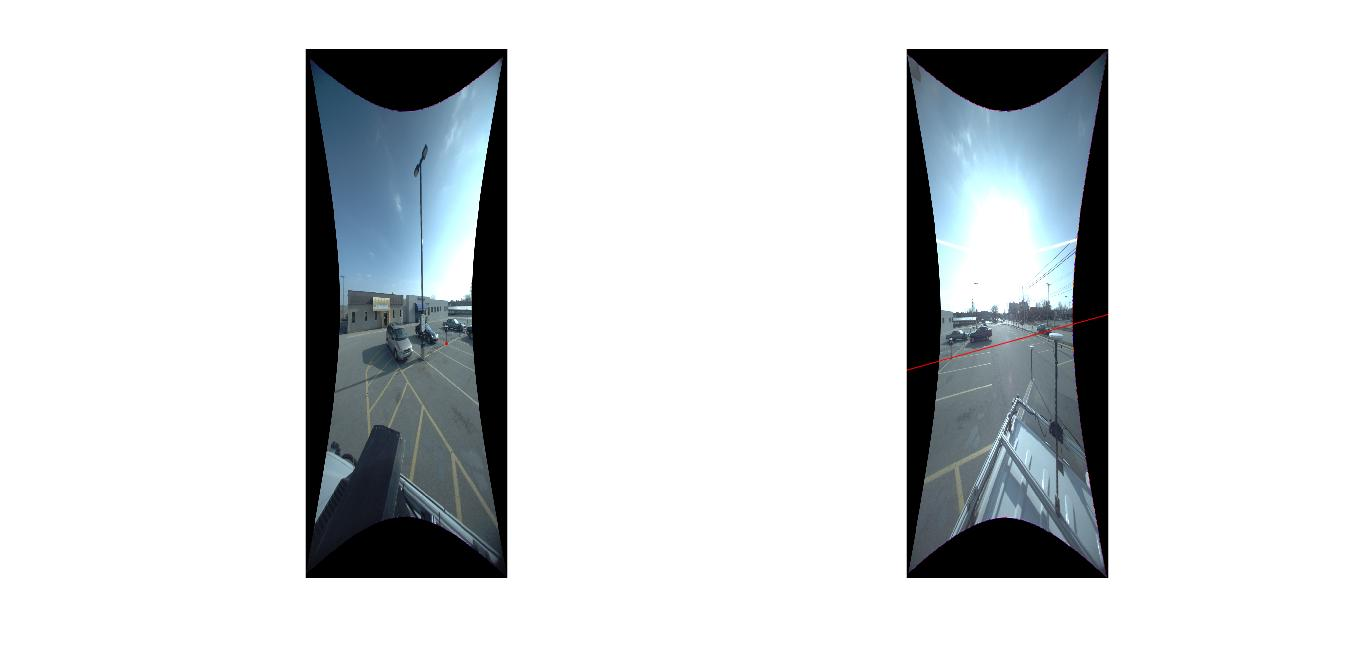
\includegraphics[scale= 0.37]{../images/q5.jpg} \\
Plot of the epipolar line correspoing to the bottom of the parking meter in camera 1.
\end{center}
\section{}
\subsection*{(a)}
Let $x_n = \begin{bmatrix}
				h_n,\ \textit{height of the object at time n$\Delta$t} \\
				v_n,\ \textit{upward velocity of the object at time n$\Delta$t }
		   \end{bmatrix}$ be the state of the object at time, $t = n \Delta t$. \\ \\
Now, the state equations to model the object's state are :
\begin{align*}
v_n & = v_0 - g n \Delta t \\
\implies\ v_n & = v_{n - 1} - g \Delta t \\
Also,\ h_n & = v_0 n \Delta t - \frac{1}{2}g (n \Delta t)^2 \\
\implies\ h_n & = h_{n - 1} + v_{n - 1} \Delta t -\frac{1}{2}g {\Delta t}^2 \\
\implies\ x_{n + 1} &  = \begin{bmatrix}
					1 & \Delta t \\
					0 &    1
				\end{bmatrix}
				x_n + 
				\begin{bmatrix}
					-\frac{1}{2}g{\Delta t}^ 2 \\
					-g \Delta t 
				\end{bmatrix} + \upvarepsilon_{n + 1}\ & where\
				\upvarepsilon_{n + 1} \sim N (0, R_n)
\end{align*}
The measurement model is given by, where $z_n$ is the measurement at time n$\Delta$t :
\begin{align*}
z_n & = \begin{bmatrix}
			1 \\
			0
		\end{bmatrix} x_n
		+ \delta_{n + 1}\ & where\ \delta_{n + 1} \sim N (0, Q_n)
\end{align*}
\subsection*{(b)}
\begin{center}
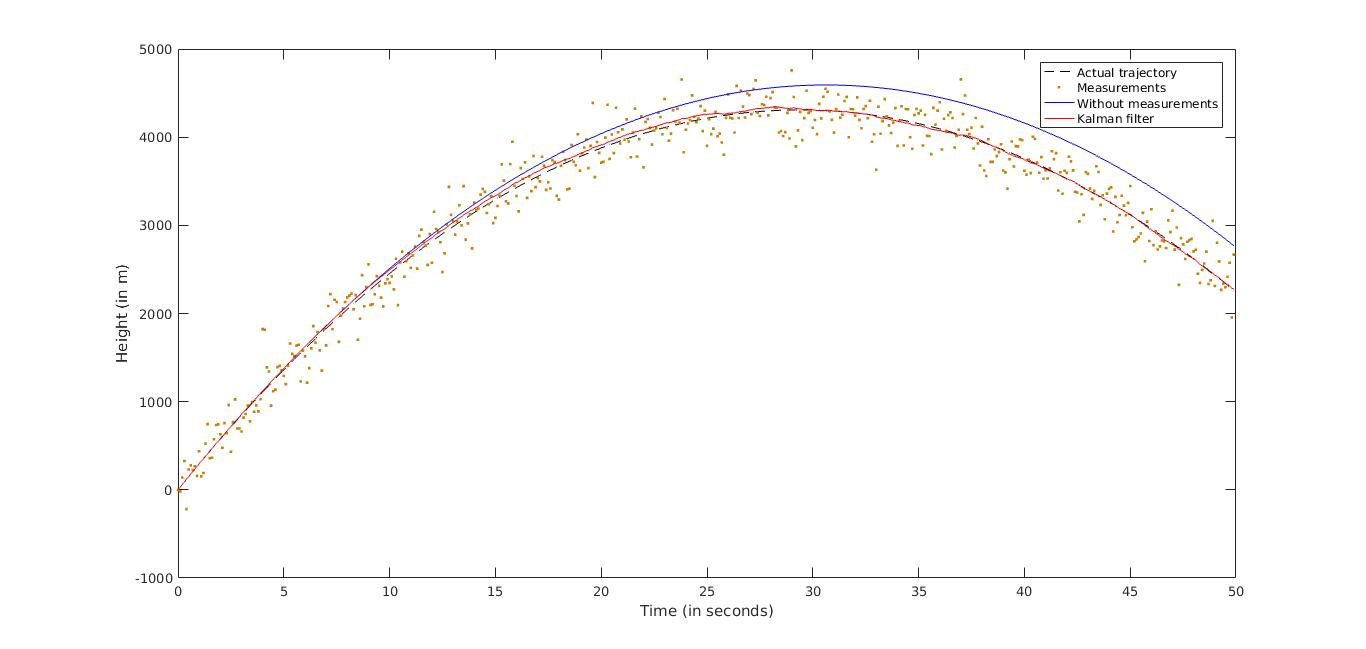
\includegraphics[scale = 0.37]{../images/q6_1.jpg} \\
\end{center}
\subsection*{(c)}
\begin{center}
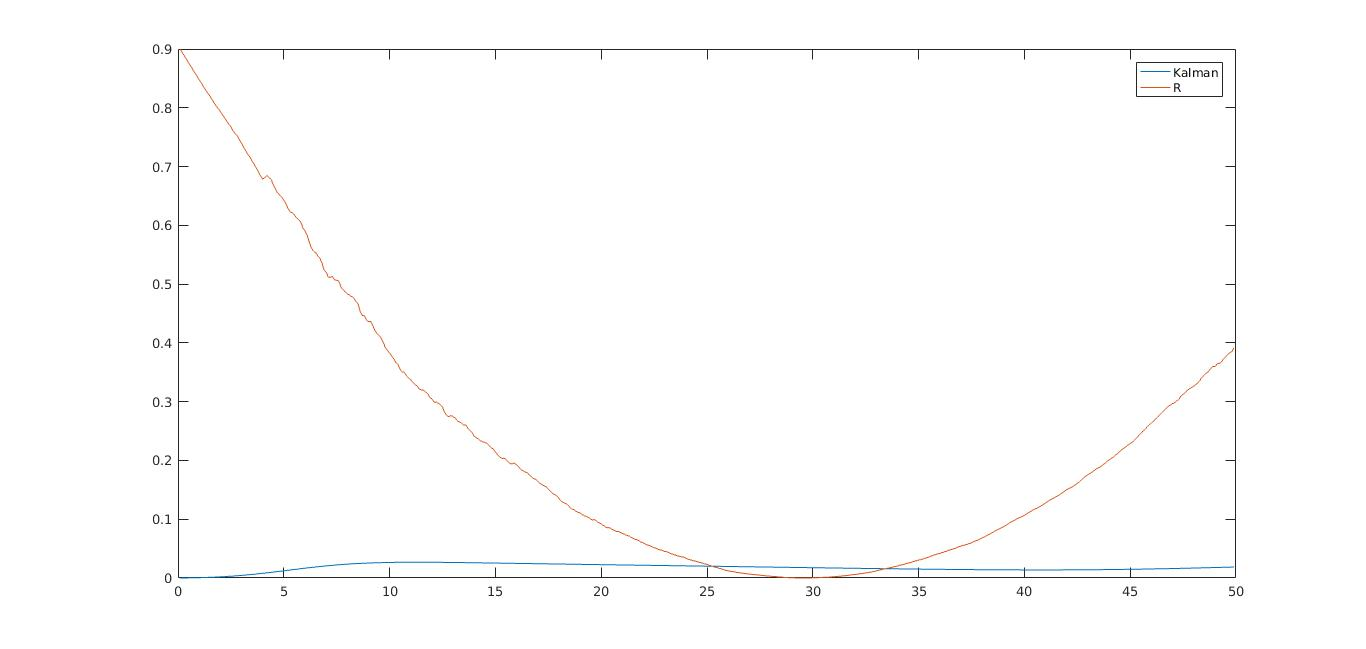
\includegraphics[scale = 0.37]{../images/q6_2.jpg} \\
\end{center}

\pagebreak
Observation : \\
I've calculated the RMSE (Root Mean Square Error) of both the orginal (with constant R) and modified (with R as a function of $||v||^2$) Kalman filters. \\
RMSE of Original = 29.4621 \\
RMSE of Modifed = 16.9210 \\
From this, one can conclude that modeling R as a function of $||v||^2$ provides a better state estimate than with the model with constant R.
\end{document}